\documentclass[tikz,border=3pt]{standalone}
% common black-and-white style of the diagrams
\usepackage[T1]{fontenc}
\usepackage{mathptmx}
\usepackage{amsmath,amssymb,bm}
\usetikzlibrary{arrows.meta,positioning,fit,calc,backgrounds,shapes.geometric,shapes.misc,patterns}
\tikzset{
  every picture/.style={font=\small, line width=0.5pt},
  >={Latex[length=2.2mm,width=1.5mm]},
  blk/.style={draw, rectangle, fill=white, align=center, inner sep=3pt, minimum height=9mm},
  grp/.style={draw, rectangle, dashed, inner sep=4pt},
  arr/.style={->, line width=0.6pt},
  darr/.style={->, line width=0.6pt, dash pattern=on 3pt off 2pt},
  lbl/.style={font=\footnotesize, align=center},
  ttl/.style={font=\small\bfseries},
}

\AtBeginDocument{\hyphenpenalty=10000 \exhyphenpenalty=10000 \relax}

\begin{document}
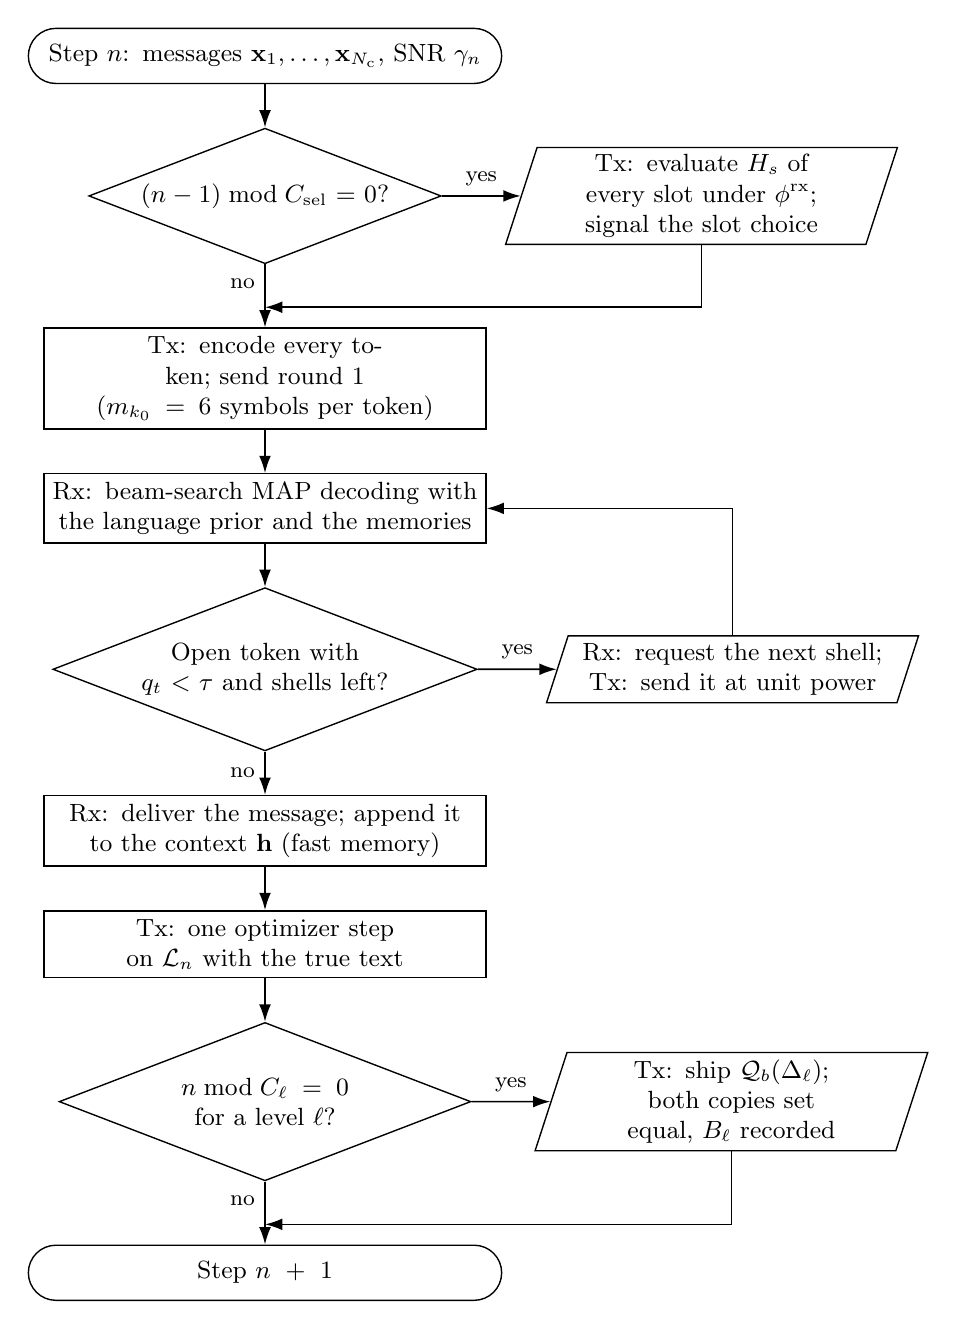
\begin{tikzpicture}[
  node distance=5.5mm,
  proc/.style={blk, text width=54mm, minimum height=8.5mm},
  io/.style={draw, trapezium, trapezium left angle=72, trapezium right angle=108, trapezium stretches body, fill=white, align=center, inner sep=2.5pt, text width=40mm, minimum height=8.5mm},
  term/.style={draw, rectangle, rounded corners=3.5mm, fill=white, align=center, inner sep=3pt, minimum height=7mm, text width=58mm},
  dec/.style={draw, diamond, aspect=2.6, fill=white, align=center, inner sep=1pt, text width=34mm},
]
\node[term] (start) {Step $n$: messages $\mathbf{x}_1,\dots,\mathbf{x}_{N_\mathrm{c}}$, SNR $\gamma_n$};
\node[dec, below=of start] (d1) {$(n-1) \bmod C_\mathrm{sel} = 0$?};
\node[io, right=10mm of d1] (slot) {Tx: evaluate $H_s$ of every slot under $\phi^{\mathrm{rx}}$; signal the slot choice};
\node[proc, below=8mm of d1] (enc) {Tx: encode every token; send round 1\\ ($m_{k_0} = 6$ symbols per token)};
\node[proc, below=of enc] (dec) {Rx: beam-search MAP decoding with the language prior and the memories};
\node[dec, below=of dec] (d2) {Open token with $q_t < \tau$ and shells left?};
\node[io, right=10mm of d2] (req) {Rx: request the next shell; Tx: send it at unit power};
\node[proc, below=of d2] (ctx) {Rx: deliver the message; append it\\ to the context $\mathbf{h}$ (fast memory)};
\node[proc, below=of ctx] (learn) {Tx: one optimizer step on $\mathcal{L}_n$ with the true text};
\node[dec, below=of learn] (d3) {$n \bmod C_\ell = 0$ for a level $\ell$?};
\node[io, right=10mm of d3] (ship) {Tx: ship $\mathcal{Q}_b(\Delta_\ell)$; both copies set equal, $B_\ell$ recorded};
\node[term, below=8mm of d3] (end) {Step $n+1$};

\draw[arr] (start) -- (d1);
\draw[arr] (d1) -- node[lbl, above]{yes} (slot);
\draw[arr] (d1) -- node[lbl, left, pos=0.3]{no} (enc);
\draw[arr] (slot) |- ($(d1.south)!0.68!(enc.north)$);
\draw[arr] (enc) -- (dec);
\draw[arr] (dec) -- (d2);
\draw[arr] (d2) -- node[lbl, above]{yes} (req);
\draw[arr] (req) |- (dec.east);
\draw[arr] (d2) -- node[lbl, left]{no} (ctx);
\draw[arr] (ctx) -- (learn);
\draw[arr] (learn) -- (d3);
\draw[arr] (d3) -- node[lbl, above]{yes} (ship);
\draw[arr] (d3) -- node[lbl, left, pos=0.3]{no} (end);
\draw[arr] (ship) |- ($(d3.south)!0.68!(end.north)$);
\end{tikzpicture}
\end{document}
